\documentclass{article}
\usepackage{amsmath}
\usepackage{tikz}
\usetikzlibrary{positioning}

\begin{document}

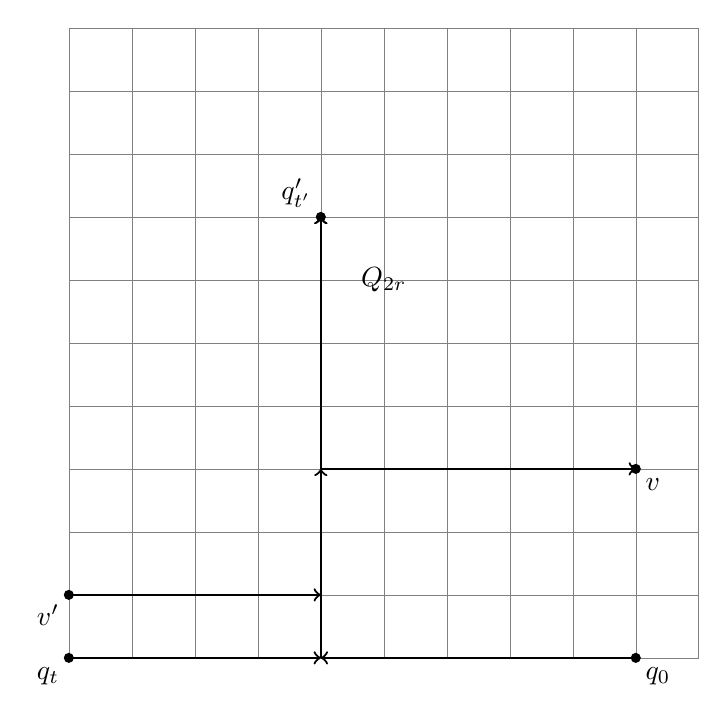
\begin{tikzpicture}[scale=0.8]
    % Draw the grid
    \draw[help lines] (0,0) grid (10,10);
    
    % Draw the highlighted cells
    \filldraw[black] (0,0) circle (2pt) node[below left] {$q_t$};
    \filldraw[black] (0,1) circle (2pt) node[below left] {$v'$};
    \filldraw[black] (9,0) circle (2pt) node[below right] {$q_0$};
    \filldraw[black] (9,3) circle (2pt) node[below right] {$v$};
    \filldraw[black] (4,7) circle (2pt) node[above left] {$q'_{t'}$};
    
    % Draw the paths
    \draw[->, thick] (0,1) -- (4,1);
    \draw[->, thick] (4,1) -- (4,7);
    \draw[->, thick] (0,0) -- (4,0);
    \draw[->, thick] (4,0) -- (4,7);
    \draw[->, thick] (9,0) -- (4,0);
    \draw[->, thick] (4,0) -- (4,3);
    \draw[->, thick] (4,3) -- (9,3);
    
    % Label the region
    \node at (5,6) {$Q_{2r}$};
\end{tikzpicture}

\end{document}